\chapter{El modelo de seguirdad de Android}
\label{chapter:background}

\section{Arquitectura de la plataforma}
\label{section:architecture}

El sistema operativo Android está compuesto por cinco capas de software, ordenadas en forma de pila
(o \textit{stack}), donde cada una de ellas provee un grupo de servicios a la capa inmediatamente
superior. De esta forma, se va abstrayendo progresivamente la interacción con el hardware (la base
de la pila) hasta llegar al nivel más alto, en el que se ubican las aplicaciones que realizarán las
tareas requeridas por los usuarios. A continuación, analizaremos brevemente cada uno de estos
niveles.

\begin{figure}
    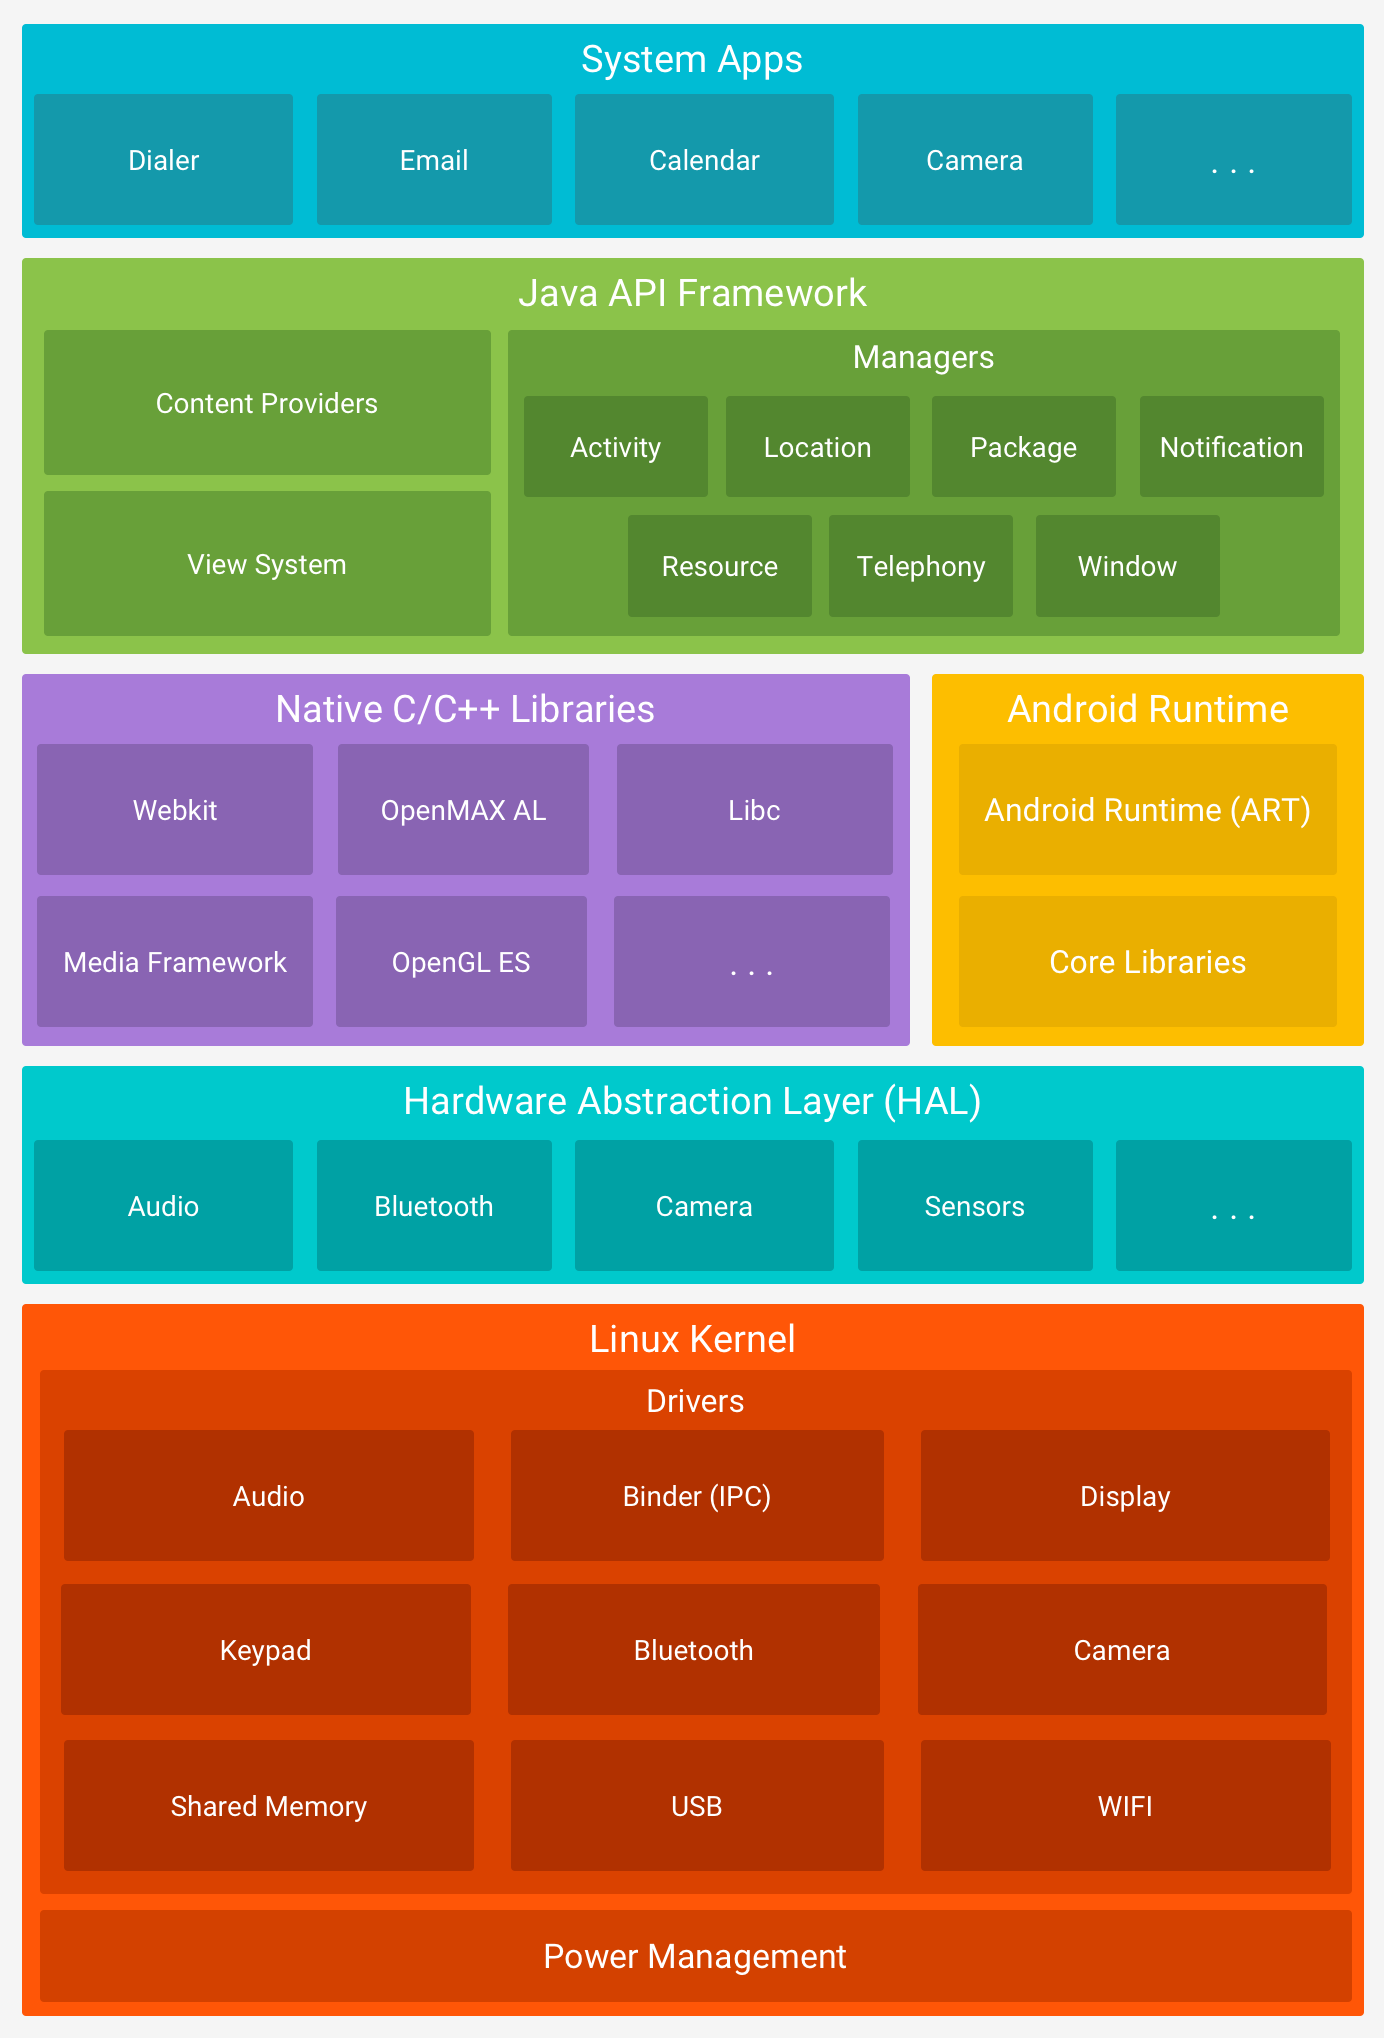
\includegraphics[scale=0.23]{imagenes/android-stack.png}
    \caption{Pila de software de Android}
    \label{fig:android_stack}
\end{figure}

\subsubsection*{Núcleo del sistema operativo: Linux}
\label{section:architecture:kernel}
La base de la plataforma Android es el \textit{kernel} de Linux. Desde el punto de vista de la
seguridad, utilizar a un núcleo tan estudiado a lo largo de los años como pilar de la arquitectura,
ayuda a generar confianza en la misma. Además, le permite a los fabricantes de dispositivos
desarrollar controladores de hardware para un sistema ya conocido.

Una de las principales utilidades de Linux de la que Android toma ventaja es del sistema de permisos
basado en usuarios\footnote{El mismo no debe confundirse con el sistema de permisos implementado por
    Android en una de las capas superiores, que es el que se formaliza y estudia en esta tesina}. Esta
característica permite que cada aplicación sea ejecutada dentro de su propia máquina virtual con un
identificador de usuario único (\texttt{UUID}) asignado a la misma. Luego, por defecto, estos
identificadores se inicializan con permisos de lectura y escritura restringidos, de manera tal que
los recursos de cada aplicación queden debidamente aislados y protegidos de potenciales
\textit{malwares}. Sin embargo, este tipo de defensa, implica la existencia de un mecanismo de
validación de referencia que arbitre las situaciones en las que una aplicación deliberadamente desee
compartir recursos con otra. Este mecanismo es implementado en las capas superiores de la
arquitectura.

Otras características de Linux utilizadas por Android son: la generación de subprocesos, la
administración de memoria de bajo nivel y otras funcionalidades encapsuladas dentro de SELinux
(\textit{\textbf{S}ecurity \textbf{E}nhanced Linux}) como la política de control de acceso
obligatorio (más conocida como \textit{MAC} por sus siglas en inglés) para distinguir entre
aplicaciones del sistema y de terceros.

\subsubsection*{Capa de abstracción de hardware}
Esta capa contiene módulos de software encargados de abstraer los diferentes componentes de
hardware, como la antena de \textit{Bluetooth} o la cámara. Estas abstracciones deben ser
independientes de los \textit{drivers} que se encuentran en el núcleo del sistema, brindando
flexibilidad y transparencia. Cada módulo está autocontenido en una librería, que es cargada
dinámicamente cuando alguna capa superior lo solicita.

\subsubsection*{Entorno de \textit{runtime} y bibliotecas nativas} En esta capa encontramos el
entorno de \textit{runtime} (o ART~\cite{art}, por sus siglas en inglés) utilizado por todas las
aplicaciones del sistema junto con algunas librerías nativas que la plataforma le ofrece a los
desarrolladores.

\subsubsection*{Marco de trabajo/API de la plataforma}
En esta capa se encuentran las interfaces que la plataforma le brinda a los desarrolladores de
aplicaciones para poder acceder a todas las funciones del sistema operativo. Es en esta capa donde
encontramos los servicios que implementan el mecanismo de validación mencionado
\hyperref[section:architecture:kernel]{previamente}.

\subsubsection*{Aplicaciones del sistema y de terceros}
Las aplicaciones representan el escalón final en esta pila de abstracciones, siendo éstas los puntos
de entrada para que cualquier usuario de Android interactúe con las funciones del dispositivo.
Algunas de estas aplicaciones ya vienen preinstaladas en la plataforma (como la de mensajería SMS o
la encargada de brindar la interfaz de configuración del sistema) mientras que otras pueden ser
instaladas a través de la tienda oficial o manualmente.


\section{Conceptos preliminares}
\label{section:preliminary}
El mecanismo que arbitra el acceso a los recursos de las aplicaciones está fuertemente basado en las
interacciones entre las mismas. Por eso, en esta sección introduciremos algunos conceptos que serán
necesarios para un mejor entendimiento del sistema.

\subsection{Componentes de una aplicación}
\label{section:preliminary:components}
Las aplicaciones de Android están conformadas por distintas piezas, que a pesar de ser funcionales
por sí mismas, interactúan entre ellas para otorgar al usuario la funcionalidad esperada. Por
ejemplo, en una aplicación que reproduce música, existirá un componente que se encargará de
presentar la interfaz al usuario mientras que otro, independiente de la interfaz, será el encargado
de reproducir la pista seleccionada. De esta manera, es posible la reproducción de una canción en
segundo~plano\footnote{Una aplicación se considera en segundo plano cuando se está ejecutando a
    pesar de no ser la aplicación que actualmente se está mostrando en la pantalla.}.

Existen cuatro tipos de componentes. Cada uno de ellos representa un punto de entrada por el cual el
sistema o el usuario pueden comunicarse con la aplicación y tiene un ciclo de vida distinto. A
continuación, describiremos brevemente cada uno de ellos.

\paragraph{Actividades:}
Una \textit{actividad} es el punto de entrada de interacción con el usuario, el encargado de ubicar
los elementos en la pantalla. Una aplicación puede tener muchas actividades, cada una de ellas
representando una pantalla distinta. Continuando con el ejemplo de la aplicación para reproducir
música, podríamos pensar que la pantalla del reproductor y la del buscador de canciones son dos
actividades distintas.

\paragraph{Servicios:}
Un \textit{servicio} permite ejecutar procesos en segundo plano. En general, es el encargado de la
ejecución de procesos largos, que de ser interrumpidos podrían afectar el desempeño de la
aplicación. Los servicios son puntos de entrada generales a la aplicación, pueden ser iniciados
tanto por un usuario (a través de una actividad), por otro servicio o por el sistema operativo.

\paragraph{Receptores de anuncios: }
Un \textit{receptor de anuncios} es el componente que se encarga de recibir mensajes del sistema y
de otras aplicaciones, incluso cuando la misma no está en ejecución. Por ejemplo, esta es la forma
en la que el sistema le avisa a todas las aplicaciones que la carga de la batería es baja. Cada
aplicación establece cuáles son los mensajes de su interés, el resto de los mensajes que reciba
simplemente serán ignorados.

\paragraph{Proveedores de contenido:}
El \textit{proveedor de contenido} es el componente encargado de administrar los datos de la
aplicación que se encuentran almacenados en medios persistentes. A través de él, cualquier
aplicación autorizada puede leer o modificar dichos datos. En otras palabras, un proveedor de
contenido actúa como intermediario entre los datos persistidos y las aplicaciones: no solo la dueña
de los datos sino también todas aquellas que hayan sido previamente autorizadas. Cada recurso allí
presente se identifica con un identificador uniforme de recursos (URI).

\subsection{Interacción entre componentes}
Una característica particular de Android es que cualquier aplicación puede iniciar un componente de
otra. Por ejemplo, una aplicación que desee tomar una foto con la cámara del dispositivo, puede
hacerlo \textit{activando} el componente correspondiente de la aplicación provista por el sistema,
en lugar de implementar una nueva actividad que lo haga. Sin embargo, como los procesos de las
aplicaciones ejecutan en procesos aislados y con permisos que limitan el acceso de otras
aplicaciones, el sistema debe actuar como intermediario en la activación de un componente. Para eso,
la aplicación en cuestión debe enviar un \textit{intent} que especifique que lo que desea es iniciar
una actividad en particular. Luego, el sistema será el encargado de activar ese componente.

\subsubsection*{Intents}
Los \textit{intents} son mensajes asíncronos que permiten la comunicación entre componentes y
aplicaciones. Existen tres casos de uso principales: el inicio de una actividad, el inicio de un
servicio y la emisión de un evento, como una indicación de que la batería del dispositivo tiene baja
carga o comenzó a cargarse. Estos mensajes puede ser \textit{explícitos}, en donde el componente de
destino está especificado; o \textit{implícitos}, donde no existe un destinatario específico, pero
el mensaje conlleva la información suficiente para que el sistema encuentre algún componente
apropiado.

\subsubsection*{Filtros de intents}
\label{section:preliminary:intent-filter}
Cuando un intent es implícito, Android busca en los \textit{filtros de intents} de cada aplicación
para verificar cuales de ellas son aptas para recibir ese mensaje. Si un único filtro de intent es
compatible, la aplicación correspondiente será iniciada. Si existe más de uno, el usuario tendrá la
posibilidad de elegir qué aplicación se activará. Los filtros de intent se declaran en el
\textit{manifiesto} de la aplicación y por lo tanto, son estáticos.

\subsection{Manifiesto de la aplicación}
\label{section:preliminary:manifest}
El archivo de manifiesto de una aplicación es un documento \texttt{xml} que contiene información
estática sobre la misma. Su tarea principal es declarar cuáles son los componentes que corresponden
a la aplicación, para que de esta forma, el sistema pueda reconocerlos como tales. Algunas otras
declaraciones que se encuentran en el manifiesto son:
\begin{enumerate}
    \item El nombre del paquete de la aplicación.
    \item Los filtros de intents \hyperref[section:preliminary:intent-filter]{previamente
              mencionados}.
    \item Los aspectos de hardware y software que la aplicación utilizará, como una cámara o los
          servicios de Bluetooth.
    \item Los permisos de usuario que requiere la aplicación
\end{enumerate}

\section{Mecanismo básico de protección: permisos}
\label{section:android:permissions}
Como ya mencionamos en la sección \ref{section:architecture:kernel}, existe en Android un mecanismo
encargado de arbitrar el acceso a la información sensible de las aplicaciones y a algunos recursos
del sistema. Este mecanismo, al que a lo largo de este trabajo llamaremos \textit{sistema de
    permisos}, cumple un rol fundamental en el modelo de seguridad de Android. Este sistema fue el que
se ha estudiado en profunidad y formalizado en esta tesina.

A grandes rasgos, para que una aplicación pueda acceder a un recurso sensible, tanto del sistema
como de otra aplicación, debe haber obtenido previamente los permisos necesarios. De ser así, la
operación es realizada con éxito. Caso contrario, la aplicación debe pedirle al sistema operativo
que le otorgue el o los permisos en cuestión. Finalmente, el sistema operativo, dependiendo del
\textit{nivel de protección} de dicho permiso, puede delegar la decisión al usuario a través de
una ventana emergente. Análogamente, si un desarrollador desea proteger un recurso de su aplicación,
puede definir un nuevo permiso y establecer que el recurso solo puede ser compartido con aquellas
otras aplicaciones que cuenten con el mismo. De esta forma, nos encontramos con una primer
clasificación entre permisos: aquellos definidos por las aplicaciones para mantener sus datos
protegidos; y los definidos por el sistema, que se necesitan para ganar acceso a los recursos del
dispositivo que pueden comprometer la privacidad del usuario (como la cámara o la lista de
contactos).

Cada permiso tiene un nombre único y cuenta un nivel de protección. El nivel de protección determina
de qué forma procederá el sistema operativo cuando un permiso es solicitado. Existen tres niveles:

\begin{enumerate}
    \item \textbf{Normal:} Estos permisos pueden ser otorgados automáticamente por el sistema ya que
          se utilizan para información o recursos que tienen un riesgo muy bajo de comprometer la
          seguridad.
    \item \textbf{Peligrosos:} Los permisos de este nivel protegen recursos mucho más sensibles y
          requieren la aprobación explícita del usuario.
    \item \textbf{De misma firma:} Un permiso de este tipo se otorga solamente si la aplicación que
          lo está solicitando y la aplicación que lo declara están firmadas con el mismo
          certificado.
\end{enumerate}

A partir de la versión \texttt{6} de Android, todos los permisos peligrosos se otorgan en tiempo de
ejecución mientras que los correspondientes a los otros niveles se conceden en el momento en el que
la aplicación se instala.

Los permisos que están asociados a una misma característica de la aplicación o dispositivo,
suelen estar agrupados. Por ejemplo, tanto el permiso necesario para leer los mensajes de texto,
como el que autoriza el envío de los mismos, pertenecen a un mismo \textit{grupo de permisos}
llamado \texttt{SMS}. El principal objetivo de agrupar permisos es evitar abrumar al usuario con
preguntas sobre la concesión de los mismos. De esta forma, si una aplicación requiere un permiso
peligroso que está agrupado, el sistema le pedirá que autorice a todo el grupo. En la sección
\ref{subsection:recent-changes:grouped-permissions}, estudiaremos más en detalle qué significa
autorizar a un grupo, dependiendo de la versión de Android que se analice.

\subsection*{Delegación de permisos}
Existen dos mecanismos mediante los cuales una aplicación puede delegar sus propios permisos a otra.
El primero consiste en dejar un \texttt{Intent} pendiente, para que otra aplicación pueda tomarlo y
ejecutarlo con los permisos y la identidad de quien lo creó. El segundo método, en cambio, consiste
en que una aplicación que cuenta con permisos de escritura/lectura sobre un proveedor de contenido
puede delegar \textit{temporalmente} esos permisos a otra aplicación. Los permisos delegados serán
revocados una vez que la actividad o servicio que los recibió haya terminado su ejecución.

\section{Cambios recientes}
\label{section:recent-changes}
En esta sección analizamos informal y brevemente los cambios que fueron introducidos entre Android
Nougat (7) y Andrid 10 que tuvieron un impacto significativo en el sistema de permisos.

\subsection{Sistema de archivos}
\label{subsection:recent-changes:filesystem}
Con intención de aumentar la seguridad de las aplicaciones, el directorio privado de todas aquellas
orientadas\footnote{
    Las aplicaciones pueden estar orientadas a distintas versiones del sistema. Android utiliza esta
    configuración para determinar la compatibilidad de ciertos comportamientos nuevos.
} a una versión posterior a Android 7 tienen permisos restringidos. Solamente la aplicación dueña
puede leer, escribir y ejecutar. Esta configuración evita la fuga de metadatos de los archivos
privados, como el tamaño o su existencia. De esta forma, las aplicaciones ya no pueden otorgar
permisos de lectura/escritura a otras para compartir sus archivos, sino que deben hacerlo otorgando
permisos temporales mediante un proveedor de contenido.

El modelo de Android del cual partimos en esta tesina, ya contemplaba el otorgamiento temporal de
permisos de lectua/escritura. Además, decidimos \textbf{no} modelar el sistema de archivos de
Android en este trabajo, dado que nuestro interés se centra en estudiar propiedades más generales
relacionadas a los permisos y creemos que el modelado de un sistema de archivos require un gran
esfuerzo que no aporta hacia donde queremos llegar. Por lo tanto, no se introdujeron cambios en el
modelo con respecto a esta nueva característica.

\subsection{Comportamiento de permisos agrupados}
\label{subsection:recent-changes:grouped-permissions}
En versiones previas a Android 8, si una aplicación solicitaba un permiso agrupado y el permiso era
otorgado, el sistema también otorgaba el resto de los permisos del mismo grupo que estuvieran
declarados en el manifiesto. Este comportamiento se consideraba incorrecto ya que violaba el
principio de mínimo privilegio en la plataforma. A partir de la octava versión de Android,
este comportamiento ha cambiado. Cuando una aplicación pide un permiso agrupado y lo consigue, solo
obtiene el permiso que fue explícitamente solicitado. Sin embargo, si posteriormente desea conseguir
otro permiso perteneciente al mismo grupo, el sistema tiene autorización para otorgarlo
automáticamente. En otras palabras, cuando una aplicación solicita un permiso \textbf{peligroso}
agrupado por primera vez, el usuario será quien determine si ese permiso es otorgado o no; pero las
solicitudes posteriores de permisos del mismo grupo serán automáticamente aceptadas por el sistema.

Desde un punto de vista conceptual, este cambio es muy favorable en pos de respetar el principio de
mínimo privilegio. Sin embargo, cabe preguntarse por qué simplemente no se delega al usuario la
autorización de cada uno de los permisos peligrosos que una aplicación solicita, que desde el punto
de vista de dicho principio, es una implementación óptima. La respuesta está en la negociación que
los autores de la plataforma deben mediar entre políticas muy estrictas de seguridad y una buena
experiencia de usuario (invadir al usuario de advertencias y solicitudes no es algo favorable en ese
sentido).

A pesar de lo mencionado en el párrafo anterior, si miramos los cambios introducidos en esta versión
desde un lugar de seguridad más concreto, seguimos encontrando situaciones peligrosas como la que
describimos a continuación.

% Cabe preguntarse por qué simplemente no se El \textit{quid} de la cuestión detrás de garantizar
% automáticamente las solicitudes subsecuentes de permisos del mismo grupo es reducir la cantidad de
% alertas que se muestran en pantalla para una mejor experiencia de usuario. 
\subsubsection{Permisos peligrosos y normales en el mismo grupo}
De acuerdo a la documentación de Android, ``cualquier permiso puede pertenecer a un grupo de
permisos sin importar el nivel del protección del mismo''~\cite{android-permissions}. Sin embargo, en
ningún lugar se especifica si permisos de distintos niveles de protección (en particular, uno de
nivel normal y otro peligroso) pueden compartir el mismo grupo ni, en caso de que sea posible, cómo
debería el sistema manejar el otorgamiento automático de permisos. De aquí se desprenden algunas
preguntas interesantes:
\begin{enumerate}
    \item Dado que los permisos normales se otorgan en tiempo de instalación y sin explícita
          aprobación del usuario, ¿habilita esto el posterior otorgamiento automático de los
          permisos peligrosos del mismo grupo? ¿Se informa de esta decisión al usuario?
    \item De no ser así, ¿cómo se encarga el sistema de manejar esta situación?
\end{enumerate}
En esta tesina formalizamos el peor de los escenarios, en donde un permiso normal puede habilitar el
otorgamiento automático de un permiso peligroso sin que el usuario se entere. Este escenario sigue
siendo válido dada la especificación informal de la plataforma. Analizaremos esto formalmente en la
sección siguiente.


\subsection{Cambios en pos de la privacidad del usuario}
Tanto en Android 9 como en Android 10 se introdujeron varios cambios que apuntan a mejorar la
privacidad de los usuarios. Entre ellos, destacamos:
\begin{enumerate}
    \item Acceso limitado a los sensores del dispositivo cuando las aplicaciones se ejecutan en
          segundo plano. Por ejemplo, las aplicaciones ya no pueden acceder ni al micrófono ni a la
          cámara sin notificar al usuario.
    \item Acceso restringido al registro de llamadas y a números telefónicos.
    \item Acceso restringido a la información obtenida de un análisis de Wi-Fi.
    \item Se agregó un permiso (peligroso) para acceder a la ubicación en segundo plano.
    \item Se agregaron restricciones sobre cuándo un servicio puede empezar una actividad. De esta
          manera, se busca que el usuario tenga más control sobre lo que ve en su pantalla.
\end{enumerate}

Sin embargo, todos estos cambios son específicos a la implementación y no tienen impacto en una
representación abstracta como la nuestra.

\subsection{Chequeo de permisos en aplicaciones \textit{legacy}}
\label{subsection:recent-changes:legacy-apps}

A partir de Android 10, cuando una aplicación orientada a una versión previa a Android 6 es
ejecutada por primera vez, el usuario será alertado. Además, dado que en las versiones más viejas de
la plataforma los permisos peligrosos se otorgaban al momento de la instalación, el usuario ahora
tendrá la posibilidad de revisar los mismos antes de que la aplicación se ejecute. Este cambio
fue formalizado e incluido en nuestro modelo.


